\section{Conclusion}
%% wrap up the report. quote ALL important results. do they agree with each other
%% i.e. cubic lattice from the photo and the 90 deg vertexs of the visual inspection.

The presence of second sound was observed on an oscilloscope in liquid 
superfluid helium (\he-II) at 3.02Tor (1.46K).

The Allen-Bradley resistor used to calibrate the measurement inside the resonance chamber was calibrated at:
$$
\frac{R - (520.89\pm1.25)}{(-33.24\pm0.72)} = T
$$
for the range
$(448 \to 471)\Omega$,  $(1.4 \to 2.3)$K.
The conversion add an uncertainty of 2.17\%.

The first harmonic at 1.46K in a $72\pm1$mm tube was found at:
$$
f_1 = 72.852 \pm 0.024
$$
With the additional data of other harmonics, up to the sixth overtone, the velocity of second sound at 1.46K is measured to be:
$$v = (19.8372 \pm 0.2761) \text{ms}^{-1}$$

By following the first harmonic through a temperature
change the speed of second sound is observed to drop to zero at the transition temperature
to normalfluid from superfluid. This agrees with the theory in Equation \ref{equ:c2rsrnts2cv}.

\subsection{Furtherance}
The variable position AB resistor should have had measurements taken over the distance
to quantitatively show the node and anitnode layout inside the
resonance tube to shows a graph similar to Figure \ref{fig:proposedmesure1}.

%%pic here

\begin{figure}[htbp]
\centering
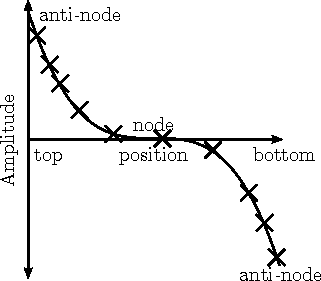
\includegraphics{pics/proposedmesure1.pdf}
\caption{Predicted results graph for the measurement of amplitude over 
position in the resonance chamber for $n=1$ harmonic.  \label{fig:proposedmesure1}}
\end{figure}

Uncertainty on the second sound propagation velocity are from the
two measured variables, frequency of the $n^\text{th}$ harmonic, and length.

The major contributor to the uncertainty 
arises from the length measurement of $72\pm1$mm. 
A more precise build of the resonance chamber would reduce this 1.38\% uncertainty.
As the uncertainty in length is from the the in-precise measurement of the ends,
a longer resonance tube would reduce the portion $\delta L / L$ used in the
uncertainty propagation calcuation for second sound velocity.

The quick method used on the $n>2$ harmonics could be 
replaced by the  graphing
method used for $n=\{1,2\}$ harmonics for more precise measurement.

The second sound disappears towards $T_B$, a slower heating method
should enable more results to be taken just under $T_B$ to show that the
frequency does drop to zero without other dominant factors.

%%probs with the experament.
